\documentclass{article} % For LaTeX2e
\usepackage{nips13submit_e,times}
\usepackage{hyperref}
\usepackage{url}
%\documentstyle[nips13submit_09,times,art10]{article} % For LaTeX 2.09

\usepackage{tikz-qtree}

%\usepackage{changepage}
%\usepackage{fancyhdr}
\usepackage{tabularx,ragged2e,booktabs,caption}

%\usepackage{graphicx}
%\usepackage{changepage}
\usepackage{amsmath, amsthm, amssymb, siunitx, url}
\usepackage[utf8]{inputenc}

\title{8-Bit Gradient Approximation for Parallelism in Deep Learning}


\author{
Tim Dettmers \\
Universià della Svizzera italiana \\
\texttt{tim.dettmers@gmail.com} }

% The \author macro works with any number of authors. There are two commands
% used to separate the names and addresses of multiple authors: \And and \AND.
%
% Using \And between authors leaves it to \LaTeX{} to determine where to break
% the lines. Using \AND forces a linebreak at that point. So, if \LaTeX{}
% puts 3 of 4 authors names on the first line, and the last on the second
% line, try using \AND instead of \And before the third author name.

\newcommand{\fix}{\marginpar{FIX}}
\newcommand{\new}{\marginpar{NEW}}

%\nipsfinalcopy % Uncomment for camera-ready version

\begin{document}


\maketitle

\begin{abstract} The application of deep learning to large data sets is important to create practical data products featuring language and visual understanding. Parallelization across processors and computers is often needed to make deep learning on large data sets feasible but bottlenecks in communication bandwidth make it difficult to attain good speedups through parallelism. Here we develop an algorithm, which provides improved utilization of the available bandwidth by compressing 32-bit gradients to 8-bit approximations. We show that these approximations do not decrease predictive performance for both model and data parallelism and provide a speedup of 2x relative to 32-bit parallelism. Thus 8-bit approximation provides an universally applicable algorithm which achieves state-of-the-art parallelism for convolutional networks.
\end{abstract}

\section{Introduction}
Deep learning is a field inherently driven by advances in computational processing (Schmidhuber, 2014). Graphics processing units (GPUs) can accelerate deep learning by a factor of up to 50 compared to a normal processor (CPU), and these speedups were integral in achieving breakthroughs in speech recognition and computer vision (Dahl et al. 2012; Krizhevsky et al. 2012). After these breakthroughs, GPUs found widespread use and many teams sought to accelerate the training of deep learning algorithms further by parallelizing the training procedure across multiple GPUs or computers (Chilimbi et al. 2014; Coates et a.2013; Dean et al. 2012; Wu et al. 2015). To make deep learning applicable and scalable for large data sets, it is important to develop successful parallel deep learning algorithms.

The parallelization of deep learning is inherently difficult. Using stochastic gradient descent (SGD) with mini-batches entails frequent synchronization of parameters across GPUs and computers with each mini-batch. Furthermore, due to the sequential nature of backpropagation, these updates must be fully completed before the next iteration of SGD can ensue (Rumelhart, Hinton, \& Williams, 1988). These two characteristics create an environment where transfer of parameters between GPUs and computers require high bandwidth and low latency for network communication. 

No viable alternative learning algorithm exists as of now which could replace SGD or backpropagation and keep the quality of the results consistent. As such the main goal in the parallelization of deep learning is to work around the bandwidth constraints induced by SGD and backpropagation. 

The most important heuristic for arm-chair evaluation of parallel algorithms in deep learning is how long the active communication $t_{\mbox{com}}$ takes compared to computation $t_{\mbox{c}}$, or more formally, how the ratio $\frac{t_{\mbox{com}}}{t_{\mbox{com}}+t_{\mbox{c}}}$ can be minimized, where $t_{\mbox{com}}$ and $t_{\mbox{c}}$, respectively. 

This heuristic can be applied in two ways: (1) Develop algorithms where computations and communication overlap so that communications are partially hidden under computation and thus the time of active communication $t_{\mbox{com}}$ is reduced; (2) develop algorithms which decrease the size of the network messages so that the efficiency of the available bandwidth is increased, thus reducing $t_{\mbox{com}}$.

In this paper we work on (2) and make the following contributions: 
 \begin{itemize}
 	\item We discuss all important hardware and software bottlenecks in model and data parallel deep learning algorithms on GPUs
 	\item We develop 8-bit gradient approximation data types and by applying them to MNIST and ImageNet show that the error rates remain unchanged despite this approximation
 	\item We show that speedup gains of 8-bit approximation compared to 32-bit gradients lie between 1.5-2.1 for common gradient dimensions in deep learning architectures
 	\item We compare our algorithm with similar work and show that 8-bit approximation sets the state-of-the-art for model parallelism in general and for data parallelism with less than 200000 parameters per layer
 \end{itemize}
\section{Background}

Here we deal with the problem of finding an algorithm which decreases the time needed for communication between neural networks on multiple GPUs in one or multiple computers. To understand the properties of a successful algorithm, it is necessary to understand how the communication between GPUs works and what the bottlenecks for both model and data parallelized deep learning architectures are. First we look at the specific properties of data and model parallelism, and then we look at general bottlenecks in GPU-to-GPU communication.

\subsection{Data parallelism}

In data parallelism, the model is kept constant for all GPUs while each GPU is fed with a different mini-batch. After each pass the gradients are exchanged, i.e. synchronized with each GPU:
 \begin{itemize} 	
 	\item How it is done: For densely connected layers, data is split by the sample dimension, e.g. for 4 GPUs, a 1024x784 mini-batch is split into four 256x784 batches; for convolutional layers the data is split by the sample dimension (better cross-validation error), or by the feature map dimension (decreases memory usage dramatically; slightly worse cross-validation error; makes architecture complicated)
 	\item Infrequent synchronization: Parameters are synchronized (averaged) once after each full forward+backward pass
 	\item Efficiency: Data parallelism is efficient when the model has few parameters, e.g. long short-term memory recurrent neural networks (Hochreiter \& Schmidhuber,1997); or the computational costs per parameter are high, e.g. convolutional layers in convolutional nets
 	\item Scaling limitations: Current GPU implementations are optimized for larger matrices so data parallelism does not scale indefinitely due to slow matrix operations (especially matrix multiplication) for small mini-batch sizes ($< 128$ per GPU); convolution implementations that rely on matrix multiplication may suffer from this too
 	\item Requires asymptotic accuracy: Good solutions can be found as long as the sequence of updates converges to the minimum asymptotically (Seide et al., 2014)
 \end{itemize}

\subsection{Model parallelism}
In model parallelism the data is kept constant for all GPUs while each GPU holds only a part of the full model:
 \begin{itemize}
 	\item How it is done: Distribute the parameters of a layer on multiple GPUs (split by input or output dimension); pass the same mini-batch through the distributed layer
 	\item Frequent synchronization: Parameters are synchronized once every layer; the outputs of the layer are either stacked or added together depending on the matrix operation
 	\item Efficiency: Model parallelism is efficient when the layer has many parameters, e.g. in densely connected layers (because the parameter matrix is reduces by a factor equal to the number of GPUs)
 	\item Scaling limitations: Poor performance for larger mini-batch sizes; the larger the mini-batch size, the larger the matrix that needs to be synchronized across GPUs
 	\item Requires numerical accuracy: Outputs must be precise as small deviation may lead to large errors in later layers; this is similar to the exploding gradient problem (Hochreiter, Bengio, Frasconi, \& Schmidhuber, 2001)
 \end{itemize}
 
\subsection{General bottlenecks}
\subsubsection{Bandwidth and latency}
GPUs within a computer communicate by using the PCI Express 3.0 (PCIe) interface which offers about 7 GB/s practical performance when a computer contains more than 2 GPUs and about 14 GB/s when it contains 2 GPUs. 

GPUs between computers usually communicate by using InfiniBand network cards which have a practical bandwidth of 3-7GB/s (quad-data-rate (QDR) and fourteen-data-rate cards (FDR), respectively).

Both PCIe and InfiniBand communication usually have about 1-2ms latency per layer for deep learning sized data transfers (as a comparison: adding two matrices for a layer of this size takes about 0.05-0.1ms). Note that both bandwidth and latency are smaller for small messages. 

Communication is the main bottleneck in deep learning which can be illustrated with a simple example: Alex-net is a convolutional network with about 60 million parameters (Krizhevsky, Sutskever, \& Hinton 2012); a full forward-backward pass is completed in under 100ms for current generation GPUs\footnote{https://github.com/soumith/convnet-benchmarks}. With 4 GPUs in naive data parallelism we need to synchronize 60 million parameters with the 3 other GPUs. Due to PCIe switches (see below) over which GPU pairs have to send their messages, this takes as long as sending 4 messages between 2 unpaired GPUs. Now 60 million 32-bit parameters take up 0.223GB of memory which at 7GB/s take 31ms for one transfer, or 124ms for a full synchronization. Adding latency for each layer, we are at more than 150ms for a full pass, which means that naive data parallelism on four GPUs would be {\it slower} than running the network on a single GPU. Thus using more GPUs or computers is not always beneficial. This also demonstrates the need for high communication bandwidth in large-scale deep learning.

\subsubsection{PCIe switches}

PCIe is built like an ordinary network where pairs of two PCIe slots share a common switch which can serve one outgoing and incoming connection simultaneously. Thus only a single device in a device-pair can communicate with another another device-pair at any one time. This holds for both GPUs and InfiniBand cards. Thus PCIe switches need to be taken into account to obtain optimal performance in a multi-GPU system.

\section{Optimal parallelism in convolutional nets}

The currently best known method to parallelize convolutional nets on N GPUs or computers is to use data parallelism in the convolutional layers and model parallelism in the dense layers (Krizhevsky, 2014). After the convolutional layers -- that is before the densely connected layers -- 1/Nth of each mini-batch are distributed across all GPUs and then a model-parallel forward and backwards pass up to the convolutional layer is performed. During each partial forward-backward pass, the next 1/Nth mini-batches are distributed across all GPUs, thus hiding the communication time for most mini-batches under the backward-pass computation time. This process is repeated N times, until all mini-batches have completed a full pass up to the convolutional layers. 

During this procedure, the gradients for the first partial forward-backward passes may be used to update the dense layers directly rather than waiting for the other N mini-batches for an average gradient. 

After this model parallelism step in the dense layers, the error-deltas for the mini-batches are passed to the respective convolutional layers, and normal data parallelism ensues from here.

\section{8-bit approximation}

We seek to develop an approximation for gradients which is small yet has sufficient accuracy to be usable for both data and model parallelism. The standard size of gradients in deep learning is 32-bit which is the smallest practical dimension for floating point numbers as CUDA only supports 32 and 64-bit floating point arithmetic. We chose to use 8-bit for our gradient approximation data type because (1) it is easy to handle as we can store it in 8-bit unsigned chars, and (2) we reasoned that less than 8-bits would have insufficient accuracy for model parallelism. 

\subsection{Designing 8-bit data types}

From these 8-bits, one bit is reserved for the sign of the number, while the rest can be used for exponent and mantissa. 

The problem with the mantissa is that our range of precision is very limited. With a 3-bit exponent the mantissa will hold values between 0 and 15 and as such decimal values over 15 will have a poor approximation and thus a large error. For example the numbers ending in 2 to 2.499 will be approximated by numbers ending in $2$ yielding an average relative error of 22.5\% in this range.

In order to decrease this error, we can use the bits of the mantissa to represent a binary tree with initial interval $(0.1,1)$ which is bisected according to the route taken through the tree; the children thus represent the start and end points for intervals in a bisection method (see Figure 1). With this method we can cover a broader range of numbers with the mantissa and can thus reduce the average relative error.

\begin{
	}[htbp]
	\centering
\tikzset{every tree node/.style={minimum width=2em,draw,circle},
	blank/.style={draw=none},
	edge from parent/.style=
	{draw, edge from parent path={(\tikzparentnode) -- (\tikzchildnode)}},
	level distance=1.5cm}
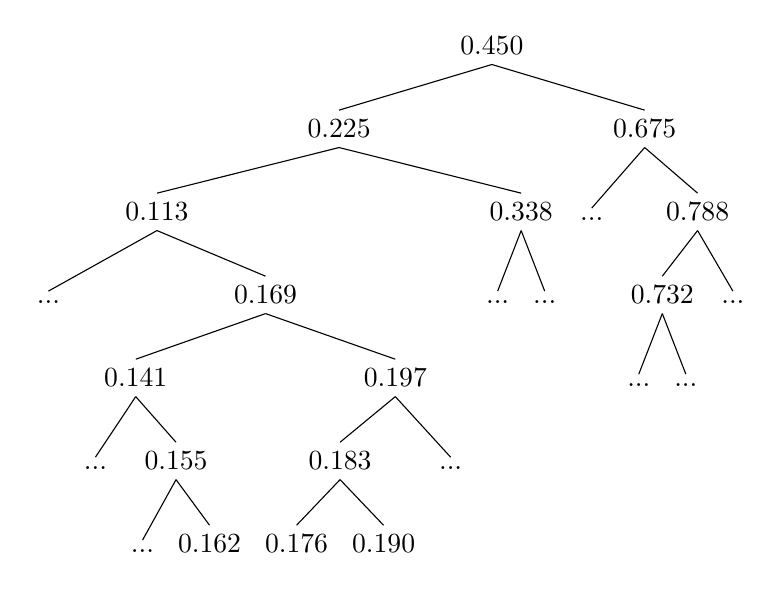
\begin{tikzpicture}
\Tree
[.0.450    
\edge[]; [.0.225 
\edge[]; [.0.113
\edge[];  {...} 
\edge[];[.0.169
\edge[];[.0.141
\edge[];  {...}
\edge[]; [.0.155
\edge[];  {...}
\edge[]; {0.162}
]
]
\edge[];[.0.197
\edge[];[.0.183
\edge[]; {0.176}
\edge[]; [.0.190 ]
]
\edge[];  {...}
]
]
]
\edge[]; [.0.338
\edge[];  {...}
\edge[];  {...}
]
]
[.0.675 
\edge[];  {...}
\edge[]; [.0.788
\edge[]; [.0.732
\edge[];  {...}
\edge[];  {...}
]
\edge[];  {...}
]
]
]
\end{tikzpicture}
\caption{Binary tree that replaces the mantissa. Each left-right decision represents one bit.}
\end{figure}

We can decrease this error further with another method: We can use additional bits from the exponent and introduce a dynamic exponent instead. This dynamic exponent may use between 0 to 7 bits, where the number $n$ of leading 0 bits represents the exponent $10^{-n}$; the first bit which is set to 1 is a flag which indicates that the next bits are part of the binary bisection tree. With this format we lose the ability to represent  large exponents (a maximum of $10^{-6}$ instead of $10^{-7}$) and we lose one bit for the binary bisection tree, but we gain the ability to approximate numbers with large absolute value with smaller error (e.g. 0.2345678 approximated as 0.236719 instead of 0.23125 or 0.2, respectively), while retaining the ability to approximate numbers with small absolute value that have few significant digits (0.0000234 approximated as 0.000019). However, one downside is that our approximation of values below $10^{-3}$ lose some accuracy because the zeros (e.g. 2 zeros and 1 flag bit) contain less information than the equivalent bits. However, gradients with absolute size greater $10^{-4}$ are more important for learning than gradients below $10^{-3}$ because they simply have a larger effect. Thus this data type should yield better training and predictive performance for deep learning algorithms. 

\begin{figure}[htbp]
	\centering
	\includegraphics[width=12cm, height=2.5cm]{types2.jpg}
	\caption{Anatomy of the three different 8-bit data types. Note that the dynamic data type shown here is a specific example and the number of bits for exponent and for the tree varies between individual numbers.}
	\label{fig:untitled}
\end{figure}

To increase the accuracy for data and model parallelism respectively, we can introduce fitting offsets for the exponent. Because model parallelism has often has larger values which have high variance, an exponent offset of $10^2$ to $10^4$ is desirable. 

For the data type with dynamic exponent, we can instead normalize a matrix by dividing by its absolute maximum value and thus transform all numbers to be in the range $[1,0]$ which is then suitable for the bisection method; upon decompression to a 32-bit float we just multiply each approximated value by the absolute maximum value to renormalize it. 

\subsection{Implementation and computational performance}

The fastest implementation for 8-bit compression and decompression we could think of is to use a binary search on a sorted table of all positive 128 values in shared GPU memory and keep track of the sign of the respective number. Shared memory is about 100 times faster than global GPU memory and thus a binary search in shared memory is very fast. 

In our implementation we used one thread per number. Additional parallelization is easily possible by dividing the table into $n$ intervals, where $n$ is the number of threads per number. However, the necessary thread synchronization is expensive and performance gains are probably negligible compared to the additional resource costs (threads). 

For decompression the table is read into shared memory and a lookup is performed for the 32-bit value for the respective 8-bit value. Here we use one thread per number/lookup.

On average, these algorithms perform compression and decompression in 1 and 0.5 nanoseconds per number, respectively, as measured on a NVIDIA GTX Titan.

The normalization of the dynamic tree data type incurs an additional performance decrease of about 0.9 nanoseconds per numbers, nearly doubling the time per number. However, we found that determining the absolute maximum value every 50 batches does not incur any significant decrease in mean test error on MNIST, $n=8, t=0.07, p= 0.94$, 99\% CIs $[0.0122.0.0129]$ and $[0.0120,0.0130]$ (t-test assumptions were satisfied). Determining the absolute maximum value every 50th batch reduces the additional overhead of normalization to 0.018 nanoseconds per number, or to a maximum of about 4\% additional time for the dynamic tree data type.

Implementations of our 8-bit approximation algorithms are available online \footnote{https://github.com/TimDettmers/clusterNet/; contact me if you need help with integrating the functions into your library}.
\newpage
\subsection{Approximation error}

As one can see from Table 1, the 8-bit dynamic tree provides the best performance for approximation numbers for random distributions and it provides the best mean absolute error in every case. 

\begin{minipage}
	{\linewidth}
	\centering
	\begin{tabular}{ cccc}
		\toprule[1.5pt]
		Distribution & Data type & Mean absolute error & Mean relative error in \%\\\midrule
		$U(0,1)$ & 8-bit dynamic tree & {\bf0.00004} & {\bf 1.39}  \\
		- & 8-bit linear quant & 0.0024 & 2.16\\
		- & 8-bit mantissa & 0.0017 & 7.22\\
		- & 8-bit static tree & 0.0007 & 4.82\\\midrule	
		$N(0,1)$ & 8-bit dynamic tree & 0.0005 }& {\bf2.46}\\
		- & 8-bit linear quant &  {\bf0.0004} & 6.47 \\
		- & 8-bit mantissa & 0.0104 & 6.89 \\
		- & 8-bit static tree & 0.0093 & 6.3 \\\midrule
		$N(0,10^2)$ & 8-bit dynamic tree & 0.049 }& {\bf2.49} \\
		- & 8-bit linear quant & {\bf0.041 }& 6.44 \\
		- & 8-bit mantissa & 1.066 & 7.19\\
		- & 8-bit static tree & 0.926 & 6.28 \\\midrule
		$N(0,0.2^2)$ & 8-bit dynamic tree & 0.000018 & {\bf2.45} \\
		- & 8-bit linear quant &{\bf 0.000015} & 6.15 \\
		- & 8-bit mantissa & 0.00055 & 8.26\\
		- & 8-bit static tree & 0.00022 & 6.58 \\\midrule
		MNIST model parallel & 8-bit dynamic tree & {\bf 0.06/0.05/0.64} & {\bf0.03/0.03/0.015} \\
		- & 8-bit linear quant & 0.06/0.08/554 & 0.03/0.02/0.09 \\
		- & 8-bit mantissa & 1.94/3.3/17.2  & 0.05/0.055/0.7\\
		- & 8-bit static tree & 0.75/1.11/13.6 &  0.04/0.043/0.054 \\\midrule
		MNIST data parallel & 8-bit dynamic tree &  ${\bf10^{-6}/10^{-7}/10^{-5}}$ &  0.04/0.07/0.055 \\
		- & 8-bit linear quant & $10^{-5}/10^{-6}/10^{-3}$ & {\bf0.02/0.03/0.025} \\
		- & 8-bit mantissa & $10^{-5}/10^{-5}/10^{-4}$ & 0.03/0.04/0.04\\
		- & 8-bit static tree & $10^{-5}/10^{-5}/10^{-3}$ &  0.025/0.04/0.04\\
		\bottomrule[1.25pt]
	\end{tabular}
	\captionof{table}{Mean absolute and relative error from a sample of size 25 million drawn from normal distributions $N(\mbox{mean},\mbox{variance})$, and the uniform distribution $U(0,1)$. The approximation of $N(0,10^2)$ was done by using an exponent offset of $10^2$ while other numbers used an exponent offset of $10^1$. For the dynamic tree the sample was divided by the maximum absolute value and then denormalized after compression.} \label{tab:title} 
	\par
	\bigskip
\end{minipage}

The mean relative error for the 8-bit dynamic tree data type may be larger for very small numbers post-normalization (this implies high variance), because it can only approximate normalized numbers with an absolute size larger than $10^{-6}$. 

When we apply all these techniques to the MNIST data set, no obvious differences in predictive performance were found for both data parallelism (see Figure 3 and 4); 95\% confidence intervals for the average minimum classification error overlap for all techniques and for both model and data parallelism indicating that no 8-bit technique is better than any other, and that results from 8-bit approximation are as good as those using 32-bit.


\begin{figure}[htbp]
	\centering
	\includegraphics[width=11cm, height=8cm]{data_parallel.png}
	\caption{Average classification test error for model parallel training of five 784x1024x1024x10 neural networks with logistic units. For each run, the neural networks were randomly initialized; dropout (0.2,0.5,0.5) and RMSProp was used.}
	\label{fig:untitled}
\end{figure}

\begin{figure}[htbp]
	\centering
	\includegraphics[width=11cm, height=8cm]{model_parallel.png}
	\caption{Average classification test error for data parallel training; here the same training parameters were used as in model parallel training in Figure 3.}
	\label{fig:untitled}
\end{figure}

We also applied to 8-bit dynamic tree data type to AlexNet on the ImageNet dataset. We used our approximation scheme for both model (dense layers) and data parallelism (convolution). Usually we have 8-bit approximation for all incoming GPUs and 32-bit gradients for the local GPU. Here we simulated training on a large GPU cluster by only using the pure 8-bit approximation gradient component by training on a single GPU. 

\begin{figure}[htbp]
	\centering
	\includegraphics[width=11cm, height=8cm]{imagenet_32vs8.png}
	\caption{Classification train and test error for the 8-bit dynamic data type used in AlexNet on the ImageNet dataset.}
	\label{fig:untitled}
\end{figure}

Figure 5 shows that the 8-bit data type does not increase the misclassification error on the train or test set for convolutional nets. Early into the training the misclassification performance is even superior to using 32-bit gradients, however, we did not run enough experiments to verify if this is due to chance or an reliable effect. The final performance on the test set was comparable to the 32-bit model: 18.65\% and 18.55\% Top5-error for the 8-bit and 32-bit model, respectively.

\newpage
\subsection{Speedup}

We measured the average total transfer time (compression, transfer, and decompression) for our techniques and compared them to 32-bit transfers between GPUs (see Figure 6). We measured this time on a board equipped with 4 GPUs which yields 8 PCIe 3.0 lanes for each GPUs and thus a theoretical bandwidth of about 8GB/s; however, bandwidth for small messages is usually considerably lower. The algorithms were run on two GTX Titans. Each matrix was transfered 100 times in this way, and the average total transfer time was measured.

We used the message passing interface (MPI) implementation provided by OpenMPI 1.8.5 which uses low level NVIDIA routines to enable GPU-to-GPU communication without the help of the CPU. MPI is commonly used to parallelize algorithms on GPU clusters.

Compressing data from 32 to 8-bit is slow for small matrices with less than 50k parameters per layer (see Figure 5), because compression and latency dominate the transfer time.\\
For messages which are larger than 250k parameters per layer, a 2x speedup in transfer speed can be achieved with 8-bit approximation compared to 32-bit data transfers. For smaller matrices, the speedup is exponentially decreasing but 8-bit transfers are always faster than 32-bit transfers.

\begin{figure}[htbp]
	\centering
	\includegraphics[width=10cm, height=8cm]{bandwidth_raw_32vs8vs1_speedups.png}
	\caption{Average transfer time for 1-bit quantization and 8-bit approximation compared to 32-bit transfers.  }
	\label{fig:untitled}
\end{figure}


\section{Comparison to other methods}

\subsection{Linear quantization}

In linear quantization a 32-bit float matrix is quantized by normalizing all numbers by the maximum magnitude in the matrix putting the values in the range [-128,127]. In our approach we normalize the values to [0,1] and map the range of these values to the 256 values of unsigned char.\\\\
Linear quantization have been used by Vanhoucke, Senior and Mao (2011) to perform fast approximate calculation on a CPU. Their optimized methods achieved near unaltered performance in a speech recognition task and increases the computational speed by roughly 25-75\%.\\\\
While GPUs currently lack the functionally to perform the fine-grained computations introduces by Vanhoucke et al., the next generation of GPUs might be capable to benefit from such implementations. In this paper we have shown that linear quantization is unsuitable for model parallelism if piecewise-linear functions -- such as the rectified linear unit -- are used, but that it can be used in data parallelism and in model parallelism if squashing functions -- such as the tanh, logistic sigmoid -- are used.


\subsection{Dynamic fixed point}

Dynamic fixed point data types are data types which use all their bits for the mantissa and have an dynamic exponent which is kept for collection of numbers (matrix, vector) and which is adjusted during run-time. Courbariaux, David and Bengio (2015) used dynamic fixed point data types with 10-bit width for computation and 12-bit width for parameter updates to train a maxout convolutional networks end-to-end. Their results on PI MNIST, MNIST, and CIFAR10 are about 20\% worse relative to the state of the art obtained by Goodfeelow and colleagues (2013).\\ 
In our work we shows that we can use 8-bit gradients for our parameter updates without degrading performance. However, dynamic fixed point datatypes can be used for end-to-end training and as such a combination of both methods might yield optimal performance for hardware that is able to utilize these data types.

\subsection{1-bit quantization}
A technique comparable to 8-bit approximation is 1-bit quantization which was developed by Seide and colleagues (2014): In 1-bit quantization each 32-bit number of the gradient is quantized to a single bit by a quantization function. This quantization function maintains a cumulative quantization error which is used to smoothen out, that is counteract the quantization error over time. The immediate error in quantization is too high to produce stable and accurate forward passes for model parallelism, but in data parallelism 1-bit quantization will converge to a local minimum seamlessly. 

In more detail, during quantization the mean of all negative and positive values, respectively, is calculated and the difference to each negative or positive number is taken. The difference between these means and respective positive or negative numbers is then taken as the cumulative quantization error. During dequantization, the positive and negative mean values are substituted for the quantized bits thus restoring local information (the means of one gradient matrix are used to restore another gradient matrix). To get a more representative global quantization, it is necessary to gather all quantized values (each GPU gathers 1/N of the data, where N is the number of GPUs), dequantize them, average them, quantize them again, and then sends them back to all other GPUs. This way the mean values are enriched with information from all available gradients, thus local information is turned into global information. This insures that the global quantization error is smoothed out over time. However, two passes are needed for this global smoothing and thus overhead and latency of quantization and transfers are larger for this technique compared to the single pass for 8-bit approximation.

In our comparison we used the 1-but quantization implementation of Torch7\footnote{https://github.com/facebook/fbcunn} (Collobert et al, 2011). The measurement then followed the same procedure as in the 8-bit case in section 4.4 where mean total transfer time was measured.

For large matrices with more than 300k parameters, 1-but quantization is about 10-20\% faster than 8-bit approximation (see Figure 5), while 8-bit approximation is notably faster for layers with less than 200k parameters like those found in the first layers of convolutional networks. However, while 1-bit quantization only works for data parallelism, 8-bit approximation also works for model parallelism which is fundamental for achieving high performance implementations of convolutional nets (Krizhevsky 2014). 

So 1-bit quantization will be more efficient for large scale GPU clusters that train large dense neural networks, while 8-bit approximation will perform favorably for convolutional nets. A combination of these techniques would also be useful, with 1-bit quantization in data parallel convolutional layers and 8-bit approximation in model parallel dense layers of a convolutional net. 

Observations by Seide an colleagues (2014) showed, that 1-bit quantization improves predictive performance compared to 32-bit methods. However it is unclear if this phenomenon is due to chance, i.e. random error, or a reliable effect. The predictive performance of 1-bit quantization thus may be on a par or slightly better than 8-bit methods.

Further advantages of 8-bit approximation include: Easy implementation which differs merely by a compression and decompression function call compared to 32-bit parallelism; and general stable approximation for a wide array of possible data generated by non-linear activation functions (see Table 1), thus making it suitable for a wide array of tasks outside of deep learning.

\section*{Conclusion}

Here we have shown that approximation of 32-bit floating point numbers with 8-bits can speed up parallel training of deep learning architectures by a factor of two while retaining predictive performance. We have shown that the dynamic tree data type is able to approximate random numbers better than the static tree or mantissa data types; however, during training all techniques seem to perform equally well.

We have shown that 8-bit approximation is currently the single best algorithm for gradient compression for convolutional nets as it offers state-of-the-art performance in early data parallel convolutional layers and model parallel dense layers. 

Due to the excellent performance for all different message sizes and applicability to both model and data parallelism, 8-bit approximation constitutes an easy-to-implement, universal algorithm for parallelism in deep learning.

We expect that further important advances in parallel computing for deep learning will come from new hardware (3D GPU memory, EDR InfiniBand adoption) and new algorithms which maintain the performance of backpropagation while providing qualities which make them easier to parallelize. 


\subsubsection*{References}

\small{
	
Chilimbi, T., Suzue, Y., Apacible, J., \& Kalyanaraman, K. (2014). Project adam: Building an efficient and scalable deep learning training system. In 11th USENIX Symposium on Operating Systems Design and Implementation (OSDI 14) (pp. 571-582).

Coates, A., Huval, B., Wang, T., Wu, D., Catanzaro, B., \& Andrew, N. (2013). Deep learning with cots hpc systems. In Proceedings of The 30th International Conference on Machine Learning (pp. 1337-1345).

Collobert, R., Kavukcuoglu, K., \& Farabet, C. (2011). Torch7: A matlab-like environment for machine learning. In BigLearn, NIPS Workshop (No. EPFL-CONF-192376).

Courbariaux, M., Bengio, Y., \& David, J. P. (2014). Low precision arithmetic for deep learning. arXiv preprint arXiv:1412.7024.
	
Dahl, G. E., Yu, D., Deng, L., \& Acero, A. (2012). Context-dependent pre-trained deep neural networks for large-vocabulary speech recognition. Audio, Speech, and Language Processing, IEEE Transactions on, 20(1), 30-42.

Dean, J., Corrado, G., Monga, R., Chen, K., Devin, M., Mao, M., ... \& Ng, A. Y. (2012). Large scale distributed deep networks. In Advances in Neural Information Processing Systems (pp. 1223-1231).

Goodfellow, I. J., Warde-Farley, D., Mirza, M., Courville, A., \& Bengio, Y. (2013). Maxout networks. arXiv preprint arXiv:1302.4389.

Hochreiter, S., \& Schmidhuber, J. (1997). Long short-term memory. Neural computation, 9(8), 1735-1780.

Hochreiter, S., Bengio, Y., Frasconi, P., \& Schmidhuber, J. (2001). Gradient flow in recurrent nets: the difficulty of learning long-term dependencies.

Krizhevsky, A., Sutskever, I., \& Hinton, G. E. (2012). Imagenet classification with deep convolutional
neural networks. In Advances in neural information processing systems (pp. 1097-1105).

Krizhevsky, A. (2014). One weird trick for parallelizing convolutional neural networks. arXiv preprint
arXiv:1404.5997.

Schmidhuber, J. (2015). Deep learning in neural networks: An overview. Neural Networks, 61, 85-117.

Seide, F., Fu, H., Droppo, J., Li, G., \& Yu, D. (2014). 1-Bit Stochastic Gradient Descent and its Application to Data-Parallel Distributed Training of Speech DNNs. In Fifteenth Annual Conference of the International Speech Communication Association.

Rumelhart, D. E., Hinton, G. E., \& Williams, R. J. (1988). Learning representations by back-propagating errors. Cognitive modeling, 5, 3.

Vanhoucke, V., Senior, A., \& Mao, M. Z. (2011). Improving the speed of neural networks on CPUs. In Proc. Deep Learning and Unsupervised Feature Learning NIPS Workshop (Vol. 1).

Wu, R., Yan, S., Shan, Y., Dang, Q., \& Sun, G. (2015). Deep Image: Scaling up Image Recognition. arXiv
preprint arXiv:1501.02876.
}

\end{document}
